% Solutions to the questions in Assignment 2 of COMP6240 Relational Database
\documentclass[12pt, a4paper]{article}
\usepackage[
top=2.5cm,
bottom=2.5cm,
left=2cm,
right=2cm,
]{geometry}
\usepackage{amsmath}
\usepackage[inline]{enumitem}
\usepackage{float}
% Drawing tree
\usepackage{forest}

% no intedent
\setlength\parindent{0pt}

% New command as alias
\newcommand{\mr}{\;\rightarrow\;}
\newcommand{\ms}{\:\:}
% Use normal text in math mode
\newcommand{\mt}[1]{\text{#1}}
\newcommand{\ma}{\;\wedge\;}
\newcommand{\mo}{\;\vee\;}
\newcommand{\mne}{\;\neq\;}
\newcommand{\me}{\;=\;}
\newcommand{\mtt}[1]{\text{\textsc{#1}}}
\begin{document}

\section{EER}
\begin{figure}[H]
  \centering
    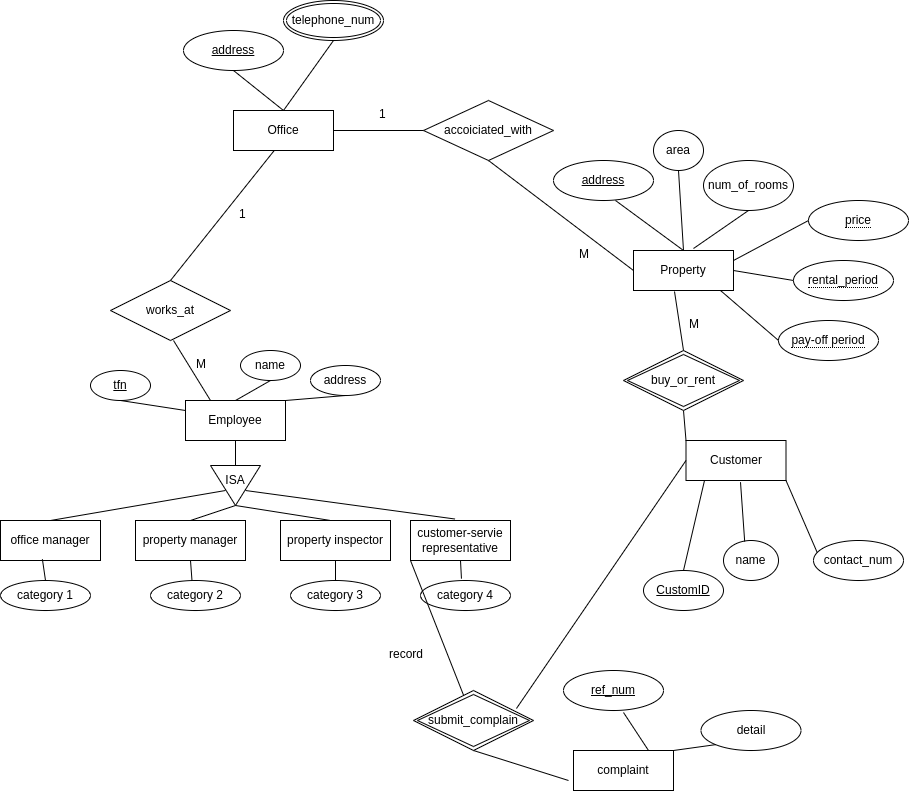
\includegraphics[width=0.8\textwidth]{Q1}
  \caption{EER for HomeComfort}
\end{figure}

\section{Solutions}
\subsection{Candidate keys}
Since each attribute appears in the dependent of all FDs in \(\Sigma\), it's impossible to decide which attribute must be part of a key.  Instead, try to build a closure of AE:
\begin{align*}
  (AE)^{+} & = AE    && \text{initialization} \\
           & = ABCE  && \text{by}\ms AE \mr BC \\
           & = ABCDE && \text{by}\ms AB \mr DE
\end{align*}
Thus, AE is a candidate key of R.  Compute the closures for other 3 FDs in \(\Sigma\) respectively:
\begin{align*}
  (B)^{+} & = B    && \text{initialization} \\
          & = AB  && \text{by}\ms B \mr A \\
          & = ABDE && \text{by}\ms AB \mr DE \\
          & = ABCDE && \text{by}\ms AE \mr BC
\end{align*}
Hence, B alone is a candidate key of R.
\begin{align*}
  (AB)^{+} & = AB    && \text{initialization} \\
          & = ABDE  && \text{by}\ms AB \mr DE \\
          & = ABCDE && \text{by}\ms AE \mr BC
\end{align*}
Hence, AB is also a candidate key of R.
\begin{align*}
  (C)^{+} & = C    && \text{initialization} \\
          & = AC  && \text{by}\ms C \mr A
\end{align*}
C is not a candidate key.

Therefore, there are 3 keys of R
\begin{itemize}[noitemsep]
\item \{A,E\}
\item \{B\}
\item \{A,B\}
\end{itemize}
The prime attributes are A, B, E; the non-prime attributes are \label{sol:1}
\subsection{Minimal cover}
1. Let \(\Sigma_{m} = \Sigma\), then make each FD in \(\Sigma_{m}\) has only a single attribute on the right hand side:
\begin{align}
  \Sigma_{m} & = \left\{AE \mr B,\right. \\
             & \qquad AE \mr C, \\
             & \qquad B \mr A, \\
  & \qquad AB \mr D, \\
  & \qquad AB \mr E, \\
  & \qquad \left. C \mr A \right \}
\end{align}
2. Try to further reduce the left hand sides of \((1), (2), (4), (5)\) FDs above such that there is only one attribute left:
\begin{align*}
  & AE \mr B && \text{AE cannot be split further} \\
  & AE \mr C && \text{same as above line} \\
  & B \mr D && \text{Drop A because B implies A and AB implies DE} \\
  & B \mr E && \text{same as above line}
\end{align*}
3. Now \(\Sigma_{m}\) becomes
\begin{align*}
  \Sigma_{m} & = \left\{AE \mr B,\right. \\
             & \qquad AE \mr C, \\
             & \qquad B \mr A, \\
             & \qquad B \mr D  \\
             & \qquad B \mr E \\
             & \qquad \left. C \mr A \right \}
\end{align*}
As mentioned above, \(B \mr A\) can further imply both \(B mr D\) and \(B mr E\), so these two are redundant.
4. A minimal cover \(\Sigma_{m}\) of \(\Sigma\) is as follows:
\begin{align*}
  \Sigma_{m} & = \left\{AE \mr B,\right. \\
             & \qquad AE \mr C, \\
             & \qquad B \mr A, \\
             & \qquad\left.C \mr A \right \}
\end{align*}

\subsection{3NF}
According to the solution of question \ref{sol:1}, although A is a prime attribute, C is not a superkey. Therefore R does \emph{not} satisfy 3NF.

Achieve a 3NF decomposition for R as follows:
\begin{enumerate}[noitemsep]
\item From \(\Sigma_{m}\), add \(R_{1}\) = \{A, E, B\}; \(R_{2}\) = \{A, E, C\}; \(R_{3}\) = \{B, A\} and \(R_{4}\) = \{C, A\} to S
\item Since \(R_{1}\) is a superkey, there is no need to add a key. Thus, S = \{\(R_{1}\), \(R_{2}\), \(R_{3}\), \(R_{4}\)\} \label{step:2}

\begin{itemize}
\item \(R_{1}\) with \(\Sigma_{1}\) = \{AE\} \(\rightarrow\) \{B\}
\item \(R_{2}\) with \(\Sigma_{2}\) = \{AE\} \(\rightarrow\) \{C\}
\item \(R_{3}\) with \(\Sigma_{3}\) = \{B\} \(\rightarrow\) \{A\}
\item \(R_{4}\) with \(\Sigma_{4}\) = \{C\} \(\rightarrow\) \{A\}
\end{itemize}
\item The FDs in step \ref{step:2} (\(\Sigma_{1} \cup \Sigma_{2} \cup \Sigma_{3} \cup \Sigma_{4}\)) is equivalent to \(\Sigma\).
\end{enumerate}

\section{Solutions}
To check if \textsc{Meeting} in BCNF, first step is to identify the key(s).  Since Client, Date, and Branch do not appear in dependent of any FDs in \(\Sigma\), they must be part of the key(s).  Start to build closure of them

% Use tabluar to align steps
\vspace{2ex}
\hspace*{\fill}%
\begin{tabular}{l@{\hskip 0.1in}c@{\hskip 0.1in}l@{\hskip 0.5in}|r@{}p{3in}}
 (Branch, Client, Date)$^{+}$ & = & Branch, Client, Date, Room &  by FD3 \\
 & = & Branch, Client, Date, Room, Employee &  by FD2 \\
\end{tabular}%
\hspace*{\fill}
\vspace{2ex}

Since in FD1, FD2, and FD4, all their left hand sides are\emph{not} superkeys, \textsc{Meeting} is \emph{not} in BCNF.


\section{Solutions}
\subsection{Relational algebra queries}
\subsubsection{a}
\begin{align*}
  & R_{1} := \pi_{\mt{StaffID}}(\text{STAFF}) \\
  & R_{2} := \pi_{\mt{StaffID}}(\sigma_{\mt{HNm}=\mt{`PeralOrient'}}(\rho_{(\mt{CID,StaffID,HNm,RNo,Date,Cost})}(\text{BOOKING}))) \\
  & Result = R_{1} - R_{2}
\end{align*}
\subsubsection{b}
\begin{align*}
  & R_{1} := \sigma_{\mt{Date} \me \mt{`27-09-2023'}}(\text{BOOKING}) \\
  & R_{2} := \rho_{B_{1}}(R_{1}) \times \rho_{B_{2}}(R_{1}) \\
  & R_{3} := \sigma_{(B_{1}.\mt{CID} \me B_{2}.\mt{CID} \ma B_{1}.\mt{HNm} \mne B_{2}.\mt{HNm}) \mo (B_{1}.\mt{CID} \me B_{2}.\mt{CID} \ma B_{1}.\mt{RNo} \mne B_{2}.\mt{RNo})}(R_{2}) \\
  & R_{4} := \rho_{B_{dups}(\mt{CID, SID, HNm, RNo, Date, Cost})}(\pi_{B_{1}.\mt{CID}, B_{1}.\mt{SID}, B_{1}.\mt{HNm}, B_{1}.\mt{RNo}, B_{1}.\mt{Date}, B_{1}.\mt{Cost}}(R_{3})) \\
  & R_{5} := R_{1} - R_{4} \\
  & R_{6} := \pi_{\mt{CustomerID}}(\rho_{(\mt{CustomerID,SID,HNm,RNo,Date,Cost})}(R_{5})) \\
  & Result = \pi_{(\mt{CustomerID,FirstName,LastName})}(R_{6} \bowtie (\mt{CUSTOMER}))
\end{align*}

\subsection{Optimization and query trees}
\subsubsection{Query tree before optimization}
\begin{forest}
  [\(\pi_{\mt{\textit{CustomerID,FirstName,LastName,Date,HNm}}}\)
  [\( \sigma_{(\mt{\textit{CID}}=\mt{\textit{CustomerID}}) \ma (\mt{\textit{HNm}}=\mt{\textit{HotelName}}) \ma (\mt{\textit{RNo}}=\mt{\textit{RoomNo}}) \ma (\mt{\textit{Cost}} > 150)}\)
  [\(\times\)
  [\textsc{Customer}]
  [\(\times\)
  [\textsc{Booking}]
  [\textsc{Hotel}]
  ]
  ]
  ]
  ]
\end{forest}

\subsubsection{Optimization}
The query is looking for those customers who booked a hotel room that costs over 150.

First, \textsc{Hotel} can be removed because
\begin{enumerate*}[label={\alph*.},font={\bfseries}]
\item All Hotel info in \textsc{Booking} is either a subset of or equal to \textsc{Hotel} and
\item the result only requires hotel names.
\end{enumerate*}
Thus, according to semantic query optimization, removing \textsc{Hotel} won't affect the result as \textsc{Booking} contains all the needed hotel names already.

Now the original RA query is simplified to:
\[
  \pi_{\mt{\textit{CustomerID,FirstName,LastName,Date,HNm}}}( \sigma_{(\mt{\textit{CID}}=\mt{\textit{CustomerID}}) \ma (\mt{\textit{Cost}} > 150)}(\mtt{Customer} \times \mtt{Booking}))
\]
\begin{enumerate}
\item push down selection \(\sigma_{(\mt{\textit{CID}}=\mt{\textit{CustomerID}}) \ma (Cost>150) }\) by applying \(\sigma_{\varphi}(R_{1} \times R_{2}) \equiv R_{1} \bowtie_{\varphi} R_{2}\):
\item[]   \(\pi_{\mt{\textit{CustomerID,FirstName,LastName,Date,HNm}}}(\mtt{Customer} \bowtie_{\sigma_{(\mt{\textit{CID}}=\mt{\textit{CustomerID}} \ma Cost>150)}} \mtt{Booking})\)
\item push down projection \(\pi_{\mt{\textit{CustomerID,FirstName,LastName,Date,HNm}}}\) by applying
\item[] \(\pi_{X}(R_{1} \bowtie R_{2}) \equiv \pi_{X}(\pi_{X_{1}}(R_{1}) \bowtie \pi_{X_{2}}(R_{2}))\):
\item[]   \((\pi_{\mt{\textit{CustomerID,FirstName,LastName}}}(\mtt{Customer})) \bowtie_{\sigma_{(\mt{\textit{CID}}=\mt{\textit{CustomerID}} \ma Cost>150)}} (\pi_{\mt{\textit{CID,Date,HNm,Cost}}}(\mtt{Booking}))\)
\end{enumerate}
\subsubsection{Query tree after optimization}
\begin{forest}
[\(\bowtie_{\mt{\textit{CID}}=\mt{\textit{CustomerID}} \ma Cost>150}\)
[\(\pi_{\mt{\textit{CustomerID,FirstName,LastName}}}\)[\textsc{Customer}]]
[\(\pi_{\mt{\textit{CID,Date,HNm,Cost}}}\)[\textsc{Booking}]]
]
\end{forest}

\end{document}
